\documentclass[main.tex]{subfiles}
\ifxetex\else
\onlyinsubfile{\usepackage{CJKutf8}}
\fi
\begin{document}
\ifxetex\else
\begin{CJK*}{UTF8}{song}
\fi

\chapter{系统启动}
\justify
BCM2835作为系统芯片(SoC),除了CPU和内存之外,还集成了GPU、USB、UART等外设。为了减少成本,树莓派没有采用类似于IBM-PC机的BIOS固件,而是把固件保存在外置的SD/MicroSD卡中。当系统加电时,CPU处于停止状态,GPU从SoC内部的ROM芯片读取第一阶段引导程序并执行。第一阶段引导程序负责从SD卡的第一个FAT文件系统中加载第二阶段引导程序bootcode.bin,由它加载第三阶段引导程序start.elf。start.elf读取并解析配置文件config.txt,然后加载kernel.img到0x8000的内存位置。至此,GPU完成了系统引导工作,然后复位CPU,从0x8000地址开始执行代码。注意,不要被扩展名所迷惑,其实kernel.img是一个无格式的二进制可执行文件。

\section{Hello world!}
为了验证各项准备工作都已经到位,先编写一个简单程序,向串口输出“Hello world!”。首先,我们需要初始化串口,如代码\ref{code:2-1}。

\begin{code}
\captionof{listing}{chapter02/kernel/machdep.c}
\label{code:2-1}
\inputminted[firstline=6,lastline=38,linenos,numbersep=5pt,frame=lines,framesep=2mm]{c}{src/chapter02/kernel/machdep.c}
\end{code}


这个函数首先设置了串口的数据位和波特率,然后将GPIO的14和15口配置为串口的收发口。如果不理解这些代码是怎么工作的,没有关系,现在不需要深入每个细节,它们不影响对关键内容的理解。初始化完成后,可以用轮询的方式向串口输出字符。如代码\ref{code:2-2}:

\begin{code}
\captionof{listing}{chapter02/kernel/machdep.c}
\label{code:2-2}
\inputminted[firstline=40,lastline=48,linenos,numbersep=5pt,frame=lines,framesep=2mm]{c}{src/chapter02/kernel/machdep.c}
\end{code}


\par

接下来编写内核的入口,即CPU执行的第一条指令。首先,新建一个文件entry.S,注意扩展名是大写的S。GNU汇编器(gas)编译汇编文件时,对于以大写S为扩展名的汇编文件,会先对源程序用C预处理(cpp)进行预处理,而扩展名为小写s的汇编文件,不会进行预处理。文件entry.S的内容如代码\ref{code:2-3}:

\begin{code}
\captionof{listing}{chapter02/kernel/entry.S}
\label{code:2-3}
\inputminted[linenos,numbersep=5pt,frame=lines,framesep=2mm]{gas}{src/chapter02/kernel/entry.S}
\end{code}


\_entry是系统的入口点,当CPU复位时,即从\_entry开始执行,它只是简单做了一个跳转,跳到reset处开始执行。首先,我们初始化栈,因为后续的函数调用需要用栈来保存一些函数参数和局部变量。考虑到栈是向低地址增长的,我们把栈放在0x1000的位置。栈初始化完成后,立即跳转到C语言的函数cstart开始完成后续的初始化工作。细心的读者可能注意到了,cstart为什么要在前面加入一个下划线?历史上,C语言编译器在全局变量或者函数的符号前面加入一个下划线,我们保留这个传统。所以,C语言中定义的全局函数cstart,在汇编中要用\_cstart引用它。反过来也一样,如果汇编语言定义的全局变量或者函数要被C语言调用,在名字前面也要加上一个下划线。

\par
cstart函数比较简单,它首先初始化串口,波特率设置为9600,然后循环调用sys\_putchar把字符串“Hello, world!”打印出来。最后,我们通过一个无限空循环让控制停cstart函数中,如代码\ref{code:2-4}。

\begin{code}
\captionof{listing}{chapter02/kernel/machdep.c}
\label{code:2-4}
\inputminted[firstline=50,lastline=60,linenos,numbersep=5pt,frame=lines,framesep=2mm]{c}{src/chapter02/kernel/machdep.c}
\end{code}


\section{编译}
代码已经写完了,接下来我们要对它们进行编译。作为操作系统内核,编译的方法也不同于普通的应用程序。具体命令如下:
\mint[breaklines]{bat}@arm-none-eabi-gcc -Wall -O2 -nostdinc -I../include -c -o entry.o entry.S@
\mint[breaklines]{bat}@arm-none-eabi-gcc -Wall -O2 -nostdinc -ffreestanding -fleading-underscore -I../include -c -o machdep.o machdep.c@
\noindent
编译选项解释如下:
\begin{itemize}
	\item -Wall告诉编译器输出所有的警告信息。
	\item -O2表示编译时采用2级优化,如果不想优化可以用-O0代替。
	\item -nostdinc表示不要使用标准的头文件搜索目录,包括编译器自带的或宿主机操作系统的头文件。标准头文件一般是为普通应用程序准备的,不适合于操作系统内核这种独立的软件。
	\item -I../include表示把路径../include加入到头文件搜索目录。这个目录包含了编译内核需要的一些头文件。
	\item -c表示只做编译,不做链接
	\item –o entry.o告诉编译器输出的目标文件名
	\item -ffreestanding告诉编译器不要使用标准函数库,程序的入口函数也不是main。操作系统内核一般不能使用宿主机操作系统提供的库函数,而且我们的入口函数是entry.S中定义的entry,不是main。
	\item -fleading-underscore表示在C语言中定义的全局变量或函数符号的前面加一个下划线。
\end{itemize}

\section{链接}
链接的过程就是把多个目标文件组装成一个可执行程序的过程。组装的方法是把各个目标文件中代码、数据按类型依序放在一起,然后解析全局变量的相互引用和函数的互相调用关系。
\par
链接器是在链接脚本(linker script)的指示下进行工作的。对于普通应用程序,编译器会提供一些默认的链接器脚本。但是,操作系统内核不能用默认的脚本进行链接。我们需要自己编写一个链接器脚本,如代码\ref{code:2-5}所示。

\begin{code}
\captionof{listing}{chapter02/kernel/kernel.ld.in}
\label{code:2-5}
\inputminted[linenos,numbersep=5pt,frame=lines,framesep=2mm]{c}{src/chapter02/kernel/kernel.ld.in}
\end{code}


我们在脚本中使用了C语言的宏定义,因此在输入给链接器之前,先对脚本进行预处理。预处理的命令如下:
\mint{bat}@arm-none-eabi-gcc -E -P -x c-header -o kernel.ld kernel.ld.in@
\noindent
选项-E表示只做预处理,-P禁止预处理器生成额外标记,-x c-header明确告诉gcc输入文件是C头文件,而不要根据扩展名推测。有了链接器脚本,下面可以进行链接:

\mint[breaklines]{bat}@arm-none-eabi-gcc -Tkenrel.ld -nostdlib entry.o machdep.o -o kernel.elf@

\noindent
-Tkernel.ld提供了链接器脚本,-nostdlib表示不要使用默认的启动代码和标准函数库,因为它们是为普通应用程序准备的。需要特别注意的是,entry.o必须是该命令的第一个目标文件,以确保它定义的\_entry符号地址是0x8000。
\par
链接器输出的文件kernel.elf是一个ELF格式的程序文件。为了验证链接器是否生成了正确的代码,可以用objdump进行反汇编(-d),
\mint[breaklines]{bat}@arm-none-eabi-objdump -d kernel.elf@
\noindent
结果如图\ref{figure:2-1}所示。可以看出,指令从0x8000开始,右边的汇编指令与entry.S完全一致。

\begin{figure}[htp]
\centering
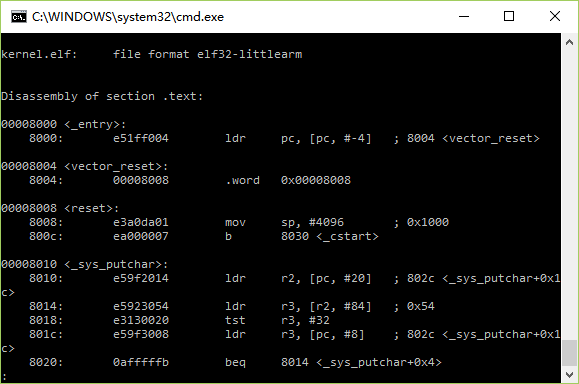
\includegraphics[scale=0.4]{figures/2-1.png}
\caption{objdump反汇编的输出}
\label{figure:2-1}
\end{figure}

树莓派只能加载无格式的二进制可执行文件,而不是ELF格式的程序文件。我们用objcopy把格式信息剥离,只留下可执行代码。命令如下:
\mint[breaklines]{bat}@arm-none-eabi-objcopy kernel.elf -O binary kernel.img@
\noindent
-O binary很显然是告诉objcopy输出不带格式的二进制文件。
\section{运行}
把kernel.img复制到SD卡根目录,并插入树莓派后加电,应该能够在串口输出中看到“Hello world!”,如图\ref{figure:2-2}所示。

\begin{figure}[htp]
\centering
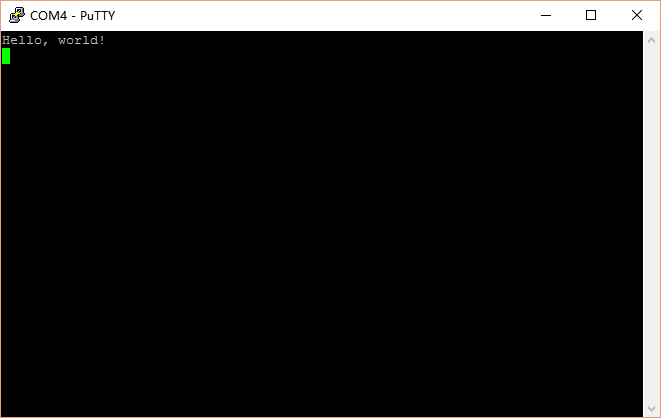
\includegraphics[scale=0.4]{figures/2-2.png}
\caption{树莓派说“Hello, world!”}
\label{figure:2-2}
\end{figure}

\section{提高开发效率}
\justify
如果看到了“Hello, world!”,那么恭喜你,开发环境已经没有问题,可以继续开发。但是,前面的编译和链接要敲很多命令,效率很低,也非常容易出错。为此,我们采用GNU make作为项目管理工具,帮我们处理繁琐、重复的工作。Make需要我们提供一个Makefie来告诉它如何完成工作。

\par
Makefile的格式其实很简单,它的每一行要么是变量定义,要么是目标(target),要么是动作(action)。动作必须从目标的下一行开始,而且行首必须是制表符(Tab),它告诉make如何根据依赖生成目标。注意,依赖本身也可以是目标,如示例中的dependency1。
\begin{figure}[htp]
\centering
\begin{minipage}{0.4\textwidth}
\begin{minted}{make}
variable=value
target: dependency1 dependency2
    action1
    action2
dependency1:dependency3
    action3
\end{minted}
\end{minipage}
\end{figure}
\par
有了Makefile,只要运行 “make target”,它会根据target的依赖,执行动作。如果依赖本身也是目标,它的动作也会被执行,形成递归执行,直到所有的依赖都得到满足。如果不带目标运行make,默认构建第一个目标。

\par
我们的Makefile如代码\ref{lst:firstLst}所示。
\begin{code}
\captionof{listing}{kernel/Makefile}
\label{lst:firstLst}
\inputminted[linenos,numbersep=5pt,frame=lines,framesep=2mm]{make}{src/chapter02/kernel/Makefile}
\end{code}
有了Makefile,我们修改源代码后,只要敲make就会生成或更新kernel.img(因为它是第一个目标),大大提高了开发效率。此外,make clean会删除所有自动生成的文件。

\section{小结}
本章我们通过实现一个非常简单功能,一方面验证了整个开发环境,另一方面也初步掌握了操作系统内核的开发流程,为后续进行更复杂的开发工作奠定了基础。

\iffalse
    \section{调试}
    为了方便调试,经常需要输出一些格式化的数据,为此我们找了第三方的函数snprintf【】来实现格式化输出的功能。注意,该函数不支持浮点数的格式化输出。

    \inputminted[linenos,numbersep=5pt,frame=lines,framesep=2mm]{c}{src/chapter02/kernel/printk.c}
\fi

\clearpage
\ifxetex\else
\end{CJK*}
\fi
\end{document} 